\begin{titlepage}

\newgeometry{top=0mm,right=20mm,left=20mm,bottom=0mm}



	%--------------------  Entete de l'Ecole ----------------------%

	\begin{figure}[t]
		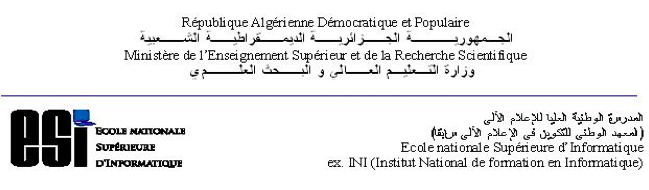
\includegraphics[scale=0.75]{ESI.png}\\[0.6in]
	\end{figure}
	
	
	
	%--------------------------------------------------------------%
	\begin{center}
	
	%------------------------  Le sujet ---------------------------%
		\LARGE \textbf{ Mémoire}\\
		\Large{
			Pour Obtention du diplôme de Master En Informatique\\
			\textbf{Option : Système Informatique (SIQ)}
			%\textsc thèse D'Ingéniorat En Informatique sous le thème :
		}\\
		\huge {
		\rule{\linewidth}{.5pt}
			\textbf{
				Méthodes d’optimisation hybrides : les heuristiques au service des méthodes exactes
			} 
			\rule{\linewidth}{.5pt}
		}\\[0.4in]
		\Large
	%--------------------------------------------------------------%	
	
	%-------------------------  Mon nom ---------------------------%
	\textbf{Réaliser par:}\\
	\begin{multicols}{}
			\Large 	Ali YADDADEN\\
			\large ea\_yaddaden@esi.dz\\
			ESI\\
		
	\end{multicols} 
	
	\vskip 0.13in
	%--------------------------------------------------------------%	

	%-----------------------  Encadreures -------------------------%
	 \textbf{Encadreur:}
	 
	 \begin{multicols}{}
			\Large 	Mme. Fatima BENBOUZID SI TAYEB\\
 			%\Large  M. Aziz MOUKRIM\\
 			%\Large  M. Jean\-Paul BOUFFLET\\
	\end{multicols}
	
	%--------------------------------------------------------------%	
	
	\small
	\vskip 0.5in
	Octobre 2018 \\
	Année Universitaire: 2018-2019\\
	
	\end{center}		
\restoregeometry
\end{titlepage}